%% bare_conf_compsoc.tex
%% V1.4a
%% 2014/09/17
%% by Michael Shell
%% See:
%% http://www.michaelshell.org/
%% for current contact information.
%%
%% This is a skeleton file demonstrating the use of IEEEtran.cls
%% (requires IEEEtran.cls version 1.8s or later) with an IEEE Computer
%% Society conference paper.
%%
%% Support sites:
%% http://www.michaelshell.org/tex/ieeetran/
%% http://www.ctan.org/tex-archive/macros/latex/contrib/IEEEtran/
%% and
%% http://www.ieee.org/

%%*************************************************************************
%% Legal Notice:
%% This code is offered as-is without any warranty either expressed or
%% implied; without even the implied warranty of MERCHANTABILITY or
%% FITNESS FOR A PARTICULAR PURPOSE! 
%% User assumes all risk.
%% In no event shall IEEE or any contributor to this code be liable for
%% any damages or losses, including, but not limited to, incidental,
%% consequential, or any other damages, resulting from the use or misuse
%% of any information contained here.
%%
%% All comments are the opinions of their respective authors and are not
%% necessarily endorsed by the IEEE.
%%
%% This work is distributed under the LaTeX Project Public License (LPPL)
%% ( http://www.latex-project.org/ ) version 1.3, and may be freely used,
%% distributed and modified. A copy of the LPPL, version 1.3, is included
%% in the base LaTeX documentation of all distributions of LaTeX released
%% 2003/12/01 or later.
%% Retain all contribution notices and credits.
%% ** Modified files should be clearly indicated as such, including  **
%% ** renaming them and changing author support contact information. **
%%
%% File list of work: IEEEtran.cls, IEEEtran_HOWTO.pdf, bare_adv.tex,
%%                    bare_conf.tex, bare_jrnl.tex, bare_conf_compsoc.tex,
%%                    bare_jrnl_compsoc.tex, bare_jrnl_transmag.tex
%%*************************************************************************


% *** Authors should verify (and, if needed, correct) their LaTeX system  ***
% *** with the testflow diagnostic prior to trusting their LaTeX platform ***
% *** with production work. IEEE's font choices and paper sizes can       ***
% *** trigger bugs that do not appear when using other class files.       ***                          ***
% The testflow support page is at:
% http://www.michaelshell.org/tex/testflow/



\documentclass[conference,compsoc]{IEEEtran}
% Some/most Computer Society conferences require the compsoc mode option,
% but others may want the standard conference format.
%
% If IEEEtran.cls has not been installed into the LaTeX system files,
% manually specify the path to it like:
% \documentclass[conference,compsoc]{../sty/IEEEtran}





% Some very useful LaTeX packages include:
% (uncomment the ones you want to load)


% *** MISC UTILITY PACKAGES ***
%
%\usepackage{ifpdf}
% Heiko Oberdiek's ifpdf.sty is very useful if you need conditional
% compilation based on whether the output is pdf or dvi.
% usage:
% \ifpdf
%   % pdf code
% \else
%   % dvi code
% \fi
% The latest version of ifpdf.sty can be obtained from:
% http://www.ctan.org/tex-archive/macros/latex/contrib/oberdiek/
% Also, note that IEEEtran.cls V1.7 and later provides a builtin
% \ifCLASSINFOpdf conditional that works the same way.
% When switching from latex to pdflatex and vice-versa, the compiler may
% have to be run twice to clear warning/error messages.






% *** CITATION PACKAGES ***
%
\ifCLASSOPTIONcompsoc
  % IEEE Computer Society needs nocompress option
  % requires .sty v4.0 or later (November 2003)
  \usepackage[nocompress]{cite}
\else
  % normal IEEE
  \usepackage{cite}
\fi
% cite.sty was written by Donald Arseneau
% V1.6 and later of IEEEtran pre-defines the format of the cite.sty package
% \cite{} output to follow that of IEEE. Loading the cite package will
% result in citation numbers being automatically sorted and properly
% "compressed/ranged". e.g., [1], [9], [2], [7], [5], [6] without using
% cite.sty will become [1], [2], [5]--[7], [9] using cite.sty. cite.sty's
% \cite will automatically add leading space, if needed. Use cite.sty's
% noadjust option (cite.sty V3.8 and later) if you want to turn this off
% such as if a citation ever needs to be enclosed in parenthesis.
% cite.sty is already installed on most LaTeX systems. Be sure and use
% version 5.0 (2009-03-20) and later if using hyperref.sty.
% The latest version can be obtained at:
% http://www.ctan.org/tex-archive/macros/latex/contrib/cite/
% The documentation is contained in the cite.sty file itself.
%
% Note that some packages require special options to format as the Computer
% Society requires. In particular, Computer Society  papers do not use
% compressed citation ranges as is done in typical IEEE papers
% (e.g., [1]-[4]). Instead, they list every citation separately in order
% (e.g., [1], [2], [3], [4]). To get the latter we need to load the cite
% package with the nocompress option which is supported by cite.sty v4.0
% and later.





% *** GRAPHICS RELATED PACKAGES ***
%
\ifCLASSINFOpdf
\usepackage[pdftex]{graphicx}
  % declare the path(s) where your graphic files are
\graphicspath{{./png}}
  % and their extensions so you won't have to specify these with
  % every instance of \includegraphics
\DeclareGraphicsExtensions{.pdf,.jpeg,.png}
\else
  % or other class option (dvipsone, dvipdf, if not using dvips). graphicx
  % will default to the driver specified in the system graphics.cfg if no
  % driver is specified.
  % \usepackage[dvips]{graphicx}
  % declare the path(s) where your graphic files are
  % \graphicspath{{../eps/}}
  % and their extensions so you won't have to specify these with
  % every instance of \includegraphics
  % \DeclareGraphicsExtensions{.eps}
\fi
% graphicx was written by David Carlisle and Sebastian Rahtz. It is
% required if you want graphics, photos, etc. graphicx.sty is already
% installed on most LaTeX systems. The latest version and documentation
% can be obtained at: 
% http://www.ctan.org/tex-archive/macros/latex/required/graphics/
% Another good source of documentation is "Using Imported Graphics in
% LaTeX2e" by Keith Reckdahl which can be found at:
% http://www.ctan.org/tex-archive/info/epslatex/
%
% latex, and pdflatex in dvi mode, support graphics in encapsulated
% postscript (.eps) format. pdflatex in pdf mode supports graphics
% in .pdf, .jpeg, .png and .mps (metapost) formats. Users should ensure
% that all non-photo figures use a vector format (.eps, .pdf, .mps) and
% not a bitmapped formats (.jpeg, .png). IEEE frowns on bitmapped formats
% which can result in "jaggedy"/blurry rendering of lines and letters as
% well as large increases in file sizes.
%
% You can find documentation about the pdfTeX application at:
% http://www.tug.org/applications/pdftex





% *** MATH PACKAGES ***
%
%\usepackage[cmex10]{amsmath}
% A popular package from the American Mathematical Society that provides
% many useful and powerful commands for dealing with mathematics. If using
% it, be sure to load this package with the cmex10 option to ensure that
% only type 1 fonts will utilized at all point sizes. Without this option,
% it is possible that some math symbols, particularly those within
% footnotes, will be rendered in bitmap form which will result in a
% document that can not be IEEE Xplore compliant!
%
% Also, note that the amsmath package sets \interdisplaylinepenalty to 10000
% thus preventing page breaks from occurring within multiline equations. Use:
%\interdisplaylinepenalty=2500
% after loading amsmath to restore such page breaks as IEEEtran.cls normally
% does. amsmath.sty is already installed on most LaTeX systems. The latest
% version and documentation can be obtained at:
% http://www.ctan.org/tex-archive/macros/latex/required/amslatex/math/





% *** SPECIALIZED LIST PACKAGES ***
%
%\usepackage{algorithmic}
% algorithmic.sty was written by Peter Williams and Rogerio Brito.
% This package provides an algorithmic environment fo describing algorithms.
% You can use the algorithmic environment in-text or within a figure
% environment to provide for a floating algorithm. Do NOT use the algorithm
% floating environment provided by algorithm.sty (by the same authors) or
% algorithm2e.sty (by Christophe Fiorio) as IEEE does not use dedicated
% algorithm float types and packages that provide these will not provide
% correct IEEE style captions. The latest version and documentation of
% algorithmic.sty can be obtained at:
% http://www.ctan.org/tex-archive/macros/latex/contrib/algorithms/
% There is also a support site at:
% http://algorithms.berlios.de/index.html
% Also of interest may be the (relatively newer and more customizable)
% algorithmicx.sty package by Szasz Janos:
% http://www.ctan.org/tex-archive/macros/latex/contrib/algorithmicx/




% *** ALIGNMENT PACKAGES ***
%
%\usepackage{array}
% Frank Mittelbach's and David Carlisle's array.sty patches and improves
% the standard LaTeX2e array and tabular environments to provide better
% appearance and additional user controls. As the default LaTeX2e table
% generation code is lacking to the point of almost being broken with
% respect to the quality of the end results, all users are strongly
% advised to use an enhanced (at the very least that provided by array.sty)
% set of table tools. array.sty is already installed on most systems. The
% latest version and documentation can be obtained at:
% http://www.ctan.org/tex-archive/macros/latex/required/tools/


% IEEEtran contains the IEEEeqnarray family of commands that can be used to
% generate multiline equations as well as matrices, tables, etc., of high
% quality.




% *** SUBFIGURE PACKAGES ***
%\ifCLASSOPTIONcompsoc
%  \usepackage[caption=false,font=footnotesize,labelfont=sf,textfont=sf]{subfig}
%\else
%  \usepackage[caption=false,font=footnotesize]{subfig}
%\fi
% subfig.sty, written by Steven Douglas Cochran, is the modern replacement
% for subfigure.sty, the latter of which is no longer maintained and is
% incompatible with some LaTeX packages including fixltx2e. However,
% subfig.sty requires and automatically loads Axel Sommerfeldt's caption.sty
% which will override IEEEtran.cls' handling of captions and this will result
% in non-IEEE style figure/table captions. To prevent this problem, be sure
% and invoke subfig.sty's "caption=false" package option (available since
% subfig.sty version 1.3, 2005/06/28) as this is will preserve IEEEtran.cls
% handling of captions.
% Note that the Computer Society format requires a sans serif font rather
% than the serif font used in traditional IEEE formatting and thus the need
% to invoke different subfig.sty package options depending on whether
% compsoc mode has been enabled.
%
% The latest version and documentation of subfig.sty can be obtained at:
% http://www.ctan.org/tex-archive/macros/latex/contrib/subfig/




% *** FLOAT PACKAGES ***
%
%\usepackage{fixltx2e}
% fixltx2e, the successor to the earlier fix2col.sty, was written by
% Frank Mittelbach and David Carlisle. This package corrects a few problems
% in the LaTeX2e kernel, the most notable of which is that in current
% LaTeX2e releases, the ordering of single and double column floats is not
% guaranteed to be preserved. Thus, an unpatched LaTeX2e can allow a
% single column figure to be placed prior to an earlier double column
% figure. The latest version and documentation can be found at:
% http://www.ctan.org/tex-archive/macros/latex/base/


%\usepackage{stfloats}
% stfloats.sty was written by Sigitas Tolusis. This package gives LaTeX2e
% the ability to do double column floats at the bottom of the page as well
% as the top. (e.g., "\begin{figure*}[!b]" is not normally possible in
% LaTeX2e). It also provides a command:
%\fnbelowfloat
% to enable the placement of footnotes below bottom floats (the standard
% LaTeX2e kernel puts them above bottom floats). This is an invasive package
% which rewrites many portions of the LaTeX2e float routines. It may not work
% with other packages that modify the LaTeX2e float routines. The latest
% version and documentation can be obtained at:
% http://www.ctan.org/tex-archive/macros/latex/contrib/sttools/
% Do not use the stfloats baselinefloat ability as IEEE does not allow
% \baselineskip to stretch. Authors submitting work to the IEEE should note
% that IEEE rarely uses double column equations and that authors should try
% to avoid such use. Do not be tempted to use the cuted.sty or midfloat.sty
% packages (also by Sigitas Tolusis) as IEEE does not format its papers in
% such ways.
% Do not attempt to use stfloats with fixltx2e as they are incompatible.
% Instead, use Morten Hogholm'a dblfloatfix which combines the features
% of both fixltx2e and stfloats:
%
\usepackage{dblfloatfix}
% The latest version can be found at:
% http://www.ctan.org/tex-archive/macros/latex/contrib/dblfloatfix/




% *** PDF, URL AND HYPERLINK PACKAGES ***
%
%\usepackage{url}
% url.sty was written by Donald Arseneau. It provides better support for
% handling and breaking URLs. url.sty is already installed on most LaTeX
% systems. The latest version and documentation can be obtained at:
% http://www.ctan.org/tex-archive/macros/latex/contrib/url/
% Basically, \url{my_url_here}.


% *** Do not adjust lengths that control margins, column widths, etc. ***
% *** Do not use packages that alter fonts (such as pslatex).         ***
% There should be no need to do such things with IEEEtran.cls V1.6 and later.
% (Unless specifically asked to do so by the journal or conference you plan
% to submit to, of course. )


% correct bad hyphenation here
\hyphenation{op-tical net-works semi-conduc-tor}















\usepackage{url}
\usepackage{framed}
\usepackage{fancyvrb}
\usepackage{listings}
\usepackage[all]{nowidow}
\lstset{
	frame=single,
	basicstyle=\ttfamily,
	breaklines
}
\usepackage{flushend}

\begin{document}
\title{14-829: Mobile Security - Fall 2015 - Assignment 3}
\author{\IEEEauthorblockN{Michael Appel}
\IEEEauthorblockA{Information Networking Institute\\
Carnegie Mellon University\\
Pittsburgh, PA\\
Email: moappel@cmu.edu}}
% make the title area
\maketitle














% As a general rule, do not put math, special symbols or citations
% in the abstract
\begin{abstract}
Android permissions are a strict set of rules for how apps can interact with a device. They technically guarantee these behaviors, but the spirit or meaning of the rule can be bypassed. For example, opening web pages without the INTERNET permission by broadcasting intents with URI. These bypasses represent large holes in Android defenses. This assignment bypasses the various \*\_LOCATION permissions in Android, and uses the WiFi signals of surrounding networks to determine a victim's location. This information is then exfiltrated via email to an attacker-controlled server. The server parses this into a GeoJSON format file, which is served on a web page displaying a custom Google map with markers of the the victim's locations.
\end{abstract}


\section{Introduction}
The use of Android permissions to secure devices does not always work as intended, which weakens the Android ecosystem as a whole. Users do not pay attention to or understand the permissions that they grant\cite{Felt:2012:APU:2335356.2335360}. Also, the meaning of the permission has been shown to be easily bypassed\cite{egners2012messing}. If an app does not request the INTERNET permission, a user does not expect it to be able to make web requests.

This assignment focuses on demonstrating the violation of this trust concerning the location permission. A malicious app is created that seemingly fetches random cat pictures for the victim's entertainment\cite{thecatapi}. The app does not request any of the coarse or fine-grained location permissions. However, it uses WiFi signals correlated with geographic WLAN broadcast data from Wigle\cite{wigle} to ascertain user location with fair accuracy.

\begin{figure}
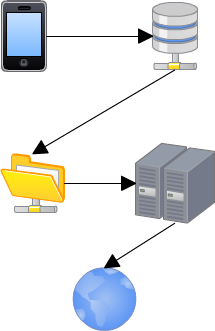
\includegraphics[width=0.5\columnwidth]{attackflow.png}
\caption{Diagram of user location being exfiltrated to a database, parsed to GeoJson, and published to the web\cite{Tracking}}
\label{FlowDiagram}
\end{figure}

The overall flow of data is shown in ~\ref{FlowDiagram} because it differs from the constraints of the assignment. Given, the large data set from Wigle, a server was setup to process incoming information from the malicious app. This exfil is stored in a database, where another process periodically picks it up to refresh a GeoJSON\cite{geojson} file. This file is then picked up by the server when anyone requests the tracking page. Thus, the app manages to track user location and publish it automatically to the internet\cite{Tracking} without using or exploiting the LOCATION permission set.

\section{App Design}
WiFilBall was designed to operate under the constraints of being stealthy about its malicious activities and being persistent about its exfiltration. Therefore, WifilBall was made to appear as a toy, and appears to load only feline photographs for entertainment. This quick entertainment ensures that the app is likely to be opened again after a reboot. In order to achieve stealth exfiltration WifilBall uses a background service WifilBat, which receives alarms to be woken up even if the screen is off.

First, it is assumed that the victim has left their phone attended in order for the app to be installed. However, in order to start the service an app must be loaded. Therefore it is also assumed that either the attacker will start the app or the user will be curious about all the possible cat pictures and start the app. Once started, the main activity launched a background thread to handle network activity for the benign appearance, and then kicks off the service in the background by calling \texttt{startService}.

Next, the WifilBat service registers listener for \texttt{ScanResults}, which handles the callbacks from the WiFi manager's scans. Originally, the app used the lightweight \texttt{Handler.postDelayed} function to reschedule itself to run every minute. At the last minute the lack of data was noticed because this function does not succeed when the device is in sleep. Therefore the app is being set to use \texttt{AlarmManager} instead of \texttt{Handler}. Currently, the main service registers the inner class \texttt{AlarmReceiver} in order to receive periodic updates. The alarm is set by the main activity with \texttt{AlarmManager\.RTC\_WAKEUP} to make sure it is running when the screen is off. Also, the timing is not inexact in order to achieve higher resolution the \texttt{setRepeating} function must be used\cite{Google:Alarms}.

\begin{figure}
  \begin{lstlisting}
1614508182556506180,0455151B1A8374....
1445546789019,24:a2:e1:f2:26:da,OLYMPUS-AIRPORT,-86
1445546789019,9c:1c:12:b7:d0:80,CMU,-67
1445546789019,9c:1c:12:b7:d0:82,CMU-GUEST,-67
1445546789019,04:bd:88:37:1d:61,CMU-GUEST,-65
1445546789019,04:bd:88:37:1d:63,CMU-SECURE,-62
1445546789019,04:bd:88:37:1d:62,eduroam,-66
1445546789019,04:bd:88:37:1d:60,CMU,-65
1445546789019,9c:1c:12:b6:c9:42,CMU-GUEST,-63
1445546789019,04:bd:88:37:1d:64,,-68
...
\end{lstlisting}
\caption{Exfiltrated email sample data}
\label{fig:email}
\end{figure}

The WifilBat service calls \texttt{WifiManager.startScan} and handles the results in a \texttt{BroadcastReceiver}. The receiver creates an authentication digest for the server since Postfix and SMTPD are piping it to a script. The email is show in \ref{fig:email}. The first line is a random number and hash (shortened for the figure). When combined with the secret, "secret squirrel", the random number string should hash out to the correct value. The email is sent out using the helper libraries included setup to use a throw-away gmail address as the sender, and the attacker account on the web server.

Finally, on the server the script parses the email and inserts all the records into a database. The schema in \ref{fig:StromOnResult} shows that duplicates are handled by the implicit uniqueness of primary key restraints. This database in turn is parsed by another script using the \texttt{last\_seen} table to extract all new timestamped data. This is converted into GeoJSON, and dumped to disk. The scripts running on the tracking web page \cite{Tracking}, will get this fresh data on every reload. There are date and time elements to filter the location of the victim within a certain window. The markers can be clicked to show the time of their signaling. Further work may include adding route lines along the path. This tool was meant to show exactly how easy and digestible personal location data could be made.

\section{Conclusion}
This app proves that location privacy can be easily violated. Within the constraints of the problem, and without using any exploits the victims location data was determined through open source data and exfiltrated. Once out of the victim's hands it came down to a worst case scenario of being published online. The app unfortunately does not work as well as intended because of the challenges with the Handler and AlarmManager at the last minute. Therefore, the data points are not as many as there should be, and the app struggles with persistence at the moment.

\begin{figure}
  \begin{lstlisting}
CREATE TABLE signals(timestamp int, bssid text, ssid text, level int, primary key(timestamp, bssid, ssid));
CREATE TABLE last_seen(id integer primary key, timestamp int);
  \end{lstlisting}
  \caption{SQLite Signals Database}
  \label{fig:StromOnResult}
\end{figure}


\begin{figure}
\begin{lstlisting}
{
 "type": "FeatureCollection",
    "features": [
        {
            "geometry": {
                "type": "Point",
                "coordinates": [
                    -79.94648743,
                    40.44424057
                ]
            },
            "type": "Feature",
            "properties": {
                "timestamp": 1445528827398
            }
        },
        {
            "geometry": {
                "type": "Point",
                "coordinates": [
                    -79.94648743,
                    40.44424057
                ]
            },
            "type": "Feature",
            "properties": {
                "timestamp": 1445528862896
            }
        },
        ...
}
\end{lstlisting}
\caption{Feature collection of points in GeoJSON format for Google Map's data layer API}
\label{geojson}
\end{figure}

\begin{figure}
\begin{lstlisting}
@Override
    protected void onCreate(Bundle savedInstanceState) {
        super.onCreate(savedInstanceState);
        setContentView(R.layout.activity_wi_fil_meow);

        /* Start the Sniffing */
        startService(new Intent(this, WifilBall.class));
        AlarmManager alarmManager = (AlarmManager) getSystemService(Context.ALARM_SERVICE);
        Intent intent = new Intent(this, WifilBall.class);
        intent.setAction("WIFIL-ALARM");
        PendingIntent pending = PendingIntent.getBroadcast(this, 0, intent, 0);
        Calendar time = Calendar.getInstance();
        time.setTimeInMillis(System.currentTimeMillis());
        alarmManager.setRepeating(AlarmManager.RTC_WAKEUP, time.getTimeInMillis(), 1000, pending);

        /* Do benign things */
        ImageView image = (ImageView) findViewById(R.id.imageView);
        AsyncTask<Void, Void, Bitmap> task = new NotMainThread().execute();
        try {
            image.setImageBitmap(task.get());
        } catch (InterruptedException | ExecutionException e) {
            Log.e("MEOW", e.toString());
            e.printStackTrace();
        }
    }
\end{lstlisting}
\caption{The main activity starts the service, alarm manager, and benign activity}
\label{wifilmeow}
\end{figure}

\clearpage
\newpage
% references section
% can use a bibliography generated by BibTeX as a .bbl file
% BibTeX documentation can be easily obtained at:
% http://www.ctan.org/tex-archive/biblio/bibtex/contrib/doc/
% The IEEEtran BibTeX style support page is at:
% http://www.michaelshell.org/tex/ieeetran/bibtex/
% argument is your BibTeX string definitions and bibliography database(s)
\bibliography{bilbo.bib}{}
\bibliographystyle{IEEEtran}
% that's all folks
\end{document}


